\section{Numerical evidence provided by \Fv s}
\label{sect:ksdim}

While mathematical approaches
provide rigorous bounds on dimensions of inertial manifolds, their
constructive description remains a challenge. In this section,
we provide numerical evidence that gives a specific integer dimension
of the inertial manifold inside the one\dmn\ \KSe.
We show that the
finite\dmn\ physical manifold can be precisely embedded in its
infinite\dmn\ \statesp, thus opening a path towards its explicit
construction. The key idea\rf{DasBuch} is to populate the inertial
manifold by an infinite hierarchy of unstable time-invariant solutions,
such as \po s, an invariant skeleton which, together
with the local ``tiles'' obtained by linearization of the dynamics,
fleshes out the physical manifold. Chaos can then be viewed as a walk on
the inertial manifold, chaperoned by the nearby unstable solutions
embedded in the physical manifold.
Unstable \po s have already been
used to compute global averages of spatiotemporally chaotic flows\rf{Christiansen97,lanCvit07,SCD07,GHCW07}.

In our analysis, we use 200 pre\po s and 200
\rpo s. These are the shortest \po s taken from the set of
over 60\,000 determined in \refref{SCD07} by near-recurrence searches.
The method preferentially finds orbits embedded in the long-time
attracting set but offers no guarantee that all orbits up to a given
period have been found.
There are infinitely many unstable orbits, and each of them
{possesses} infinitely many Floquet modes. While in the example that we
study here we do not have a detailed understanding of the organization of
\po s (their symbolic dynamics), we
show that one only needs to consider a finite number of
them to tile the physical manifold to a reasonable accuracy.
We also show, for the first time, that each local tangent tile spanned by
the \Fv s of an unstable \po\ splits into a set of
{\entangled} Floquet modes  and the remaining set of {\transient} modes.
Furthermore, we verify numerically that the {\entangled} Floquet manifold
coincides locally with the physical manifold determined by the covariant
Lyapunov vectors approach.


\subsection{Motivation from \cLvs}

Recent progress towards this aim came from numerical investigations of
the \cLvs\
of spatiotemporally chaotic flows\rf{YaTaGiChRa08,TaGiCh11}, made
possible by the
algorithms developed in \refrefs{ginelli-2007-99,WoSa07,GiChLiPo12}.
These works have revealed that the tangent space
of a generic spatially-extended dissipative system is split into two
hyperbolically decoupled subspaces: a finite\dmn\ subspace of
``entangled'' or ``physical'' Lyapunov modes (referred to in what follows
as the ``physical manifold''), which is presumed to capture all long-time
dynamics, and the remaining infinity of transient (``isolated,''
``spurious'') Lyapunov modes.
Covariant (Lyapunov) vectors span the Oseledec
subspaces\rf{lyaos,EckmannRuelle1985} and thus indicate the intrinsic
directions of growth or contraction at every point on the
physical manifold.
The dynamics of the vectors that span the physical manifold is entangled,
with frequent tangencies between them.
The {\transient} modes, on the other hand, are damped so strongly
that they are isolated - at no time do they couple by
tangencies to the {\entangled} modes.
Specifically, for domain size $L=22$,
the physical manifold consists of the leading 8 \cLvs.

It was conjectured in \refref{YaTaGiChRa08,TaGiCh11} that the physical
manifold provides a local linear approximation to the inertial manifold
at any point on the attractor, and that the dimension of the inertial
manifold is given by the number of the {\entangled} Lyapunov modes.
Further
support for this conjecture was provided by
\refref{YaRa11}, which verified that the vectors connecting pairs of
recurrent points --points on the chaotic trajectory far apart in time but
nearby each other in \statesp-- are confined within the local tangent
space of the physical manifold.

While these works showed that the physical manifold captures the
finite dimensionality of the inertial manifold, they do not tell us
much about how this inertial manifold is actually laid out in \statesp.
This is the primary reason that we instead study the set of pre/relative
\po s inside this system as they form the backbone the attractor.

\subsection{Decoupling of local Floquet exponents}

\begin{figure}[!ht]
  \centering
  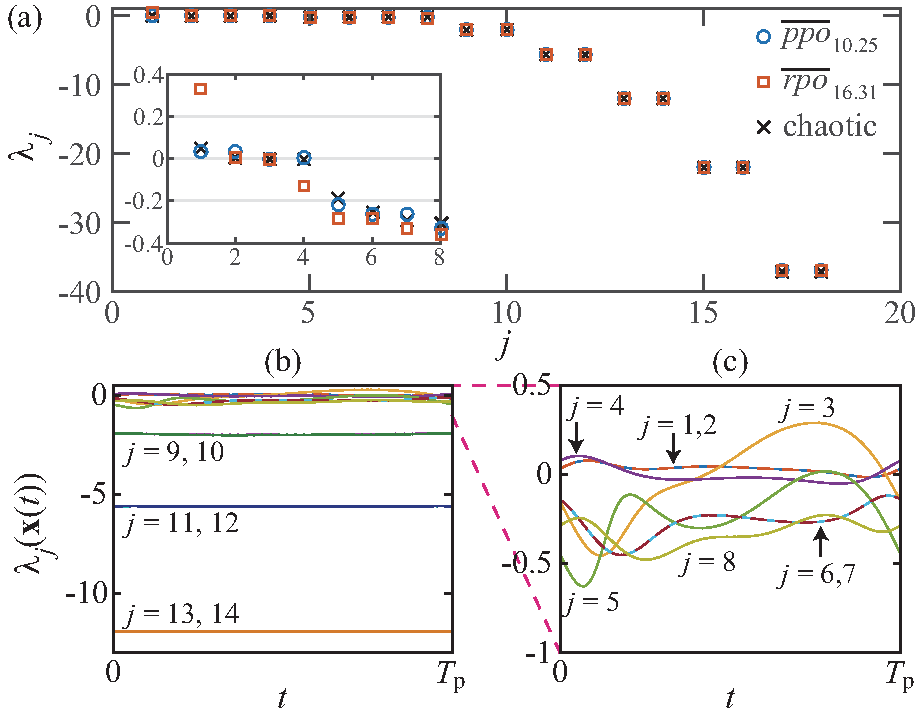
\includegraphics[width=0.9\textwidth]{ks22FloqExp}
  \caption[Local Floquet exponents of \PPO{10.25}.]{
    %(Color online)
    (a) Floquet exponents for \PPO{10.25} (circles),
    \RPO{16.31} (squares), and Lyapunov exponents of a
    chaotic trajectory (crosses).
    The inset shows a close-up of the 8 leading exponents.
    For the full Floquet spectrum of these two orbits, see
    \reftab{tab:floquet_ppo1}.
    (b) Time series of local Floquet exponents
    $\lambda_j(\ssp(t))$ for \PPO{10.25}.
    (c) Close-up of (b) showing the 8 leading exponents.
    Dashed lines indicate degenerate exponent pairs corresponding to
    complex Floquet multipliers.
  }
  \label{fig:ks22FloqExp}
\end{figure}

The definitions of Floquet exponents and \Fv s are given
in \refsect{sect:LinStab}. More specifically, for pre\po s and
\rpo s defined in \refsect{sect:kssym},
Floquet multipliers $\Lambda_j$ and vectors $\ve_j(\ssp)$ are the
eigenvalues and eigenvectors of Jacobian matrix
$J_p=R J^{\period{p}}$ or $J_p=g(\theta_{p})J^{\period{p}}$ for
pre-periodic or \rpo s, respectively, explained in \refsect{sect:kssym}.
The Floquet exponents $\lambda_j$
(if complex, we shall only consider their real parts, with multiplicity 2)
are related to multipliers by $\lambda_j=\ln|\Lambda_j|/\period{p}$.
For an orbit $(\lambda_j,\ve_j)$ denotes the $j$th Floquet
(exponent, vector); for a chaotic trajectory it denotes the
$j$th Lyapunov (exponent, vector).

\refFig{fig:ks22FloqExp}\,(a) shows the Floquet exponents spectra for the two
shortest orbits, \PPO{10.25} and \RPO{16.31},
overlaid on the Lyapunov exponents computed from a chaotic trajectory.
The basic structure of this spectrum is shared by all 400
orbits used in our study.
\footnote{
  \refRefs{YaTaGiChRa08,TaGiCh11,YaRa11} include the marginal
  Galilean symmetry mode in the mode count; here this mode is
  absent, as we have set $\int{}u(x,t)dx=0$. Consequently, the
  number of the {\entangled} modes (the dimension of the physical
  manifold) differs by one.
  \label{fn:KazzNt1}
}
For chaotic trajectories, hyperbolicity between an arbitrary pair of
Lyapunov modes can be characterized by a property called the domination
of Oseledec splitting (DOS)\rf{PuShSt04,Bochi04}.
Consider a set of finite-time Lyapunov exponents
\begin{equation}
  \lambda_j^\tau(\ssp)
  \equiv
  % \frac{1}{\tau}\ln \frac{||J^\tau(\op)\ve_j(\op)||}{||\ve_j(\op)||}
  \frac{1}{\tau}\ln ||J^\tau(\ssp)\ve_j(\ssp)||
  \,,
  \label{eq:ftle}
\end{equation}
with $L^2$ normalization $\norm{\ve_j(\ssp)}=1$.
A pair of modes $j<\ell$ is said to fulfill `DOS strict ordering'
if $\lambda_{j}^\tau(\ssp)>\lambda_{\ell}^\tau(\ssp)$
along the entire chaotic trajectory, for $\tau$ larger than some lower
bound $\tau_0$. Then this pair is guaranteed not to have
tangencies\rf{PuShSt04,Bochi04}.
For chaotic trajectories, DOS turned out to be a useful tool to
distinguish {\entangled} modes from hyperbolically decoupled {\transient}
modes\rf{YaTaGiChRa08,TaGiCh11}.
\Po s are by definition the infinite-time orbits  ($\tau$ can be any repeat
of $\period{p}$), so generically all nondegenerate pairs of modes fulfill DOS.
Instead, we find it useful to define, by analogy to the `local Lyapunov
exponent'\rf{BosPos14}, the `local Floquet exponent' as the action of
the strain rate tensor\rf{Landau59a}
\(
2\,D(\ssp) = \transp{\Mvar(\ssp)}+\Mvar(\ssp)
\)
(where $\Mvar$ is the \stabmat\ \refeq{eq:stab}) on the normalized
$j$th Floquet eigenvector,
\begin{equation}
  \lambda_{j}(\ssp)
  % = \transp{\ve_j(\ssp)} A(\ssp)\ve_j(\ssp),
  % = \Re\left[\transp{\jEigvec[j](\ssp)}\Mvar(\ssp)\jEigvec[j](\ssp)\right]
  = \transp{\ve_j(\ssp)}D(\ssp)\,\ve_j(\ssp)
  = \lim_{\tau\rightarrow 0}\lambda_j^\tau(\ssp)
  \,.
  \label{strainRateTens}
\end{equation}
We find that time series of local Floquet exponents $\lambda_j(\ssp(t))$
indicate a decoupling of the leading
`\entangled' modes from the rest of the strictly ordered, strongly
negative exponents [\reffig{fig:ks22FloqExp}\,(b) and (c)].
Another example, the local Floquet exponents of \RPO{16.31} is shown
in \reffig{fig:localFErpo1}.
Perhaps surprisingly, for every one of the 400 orbits we analyzed, the
number of the {\entangled} Floquet modes was \textit{always} 8, equal to the
previously reported number of the {\entangled} Lyapunov modes for this
system\rf{YaRa11}.
\footnote{
  see footnote \ref{fn:KazzNt1} on page \pageref{fn:KazzNt1}.
}
This leads to our first surmise: (1) each individual orbit embedded in
the attracting set carries enough information to determine the  dimension
of the physical manifold.

\begin{figure}[!ht]
  \centering
  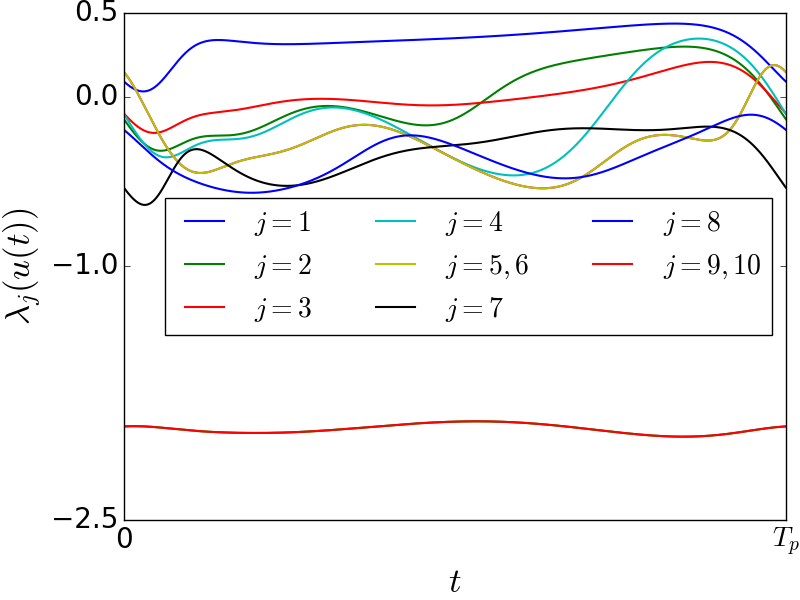
\includegraphics[width=0.7\textwidth]{localFErpo1}
  \caption[Local Floquet exponents of \RPO{16.31}.]{
    The leading 10 local Floquet exponents of \RPO{16.31} along the
    orbit for one period. The ($5$th, $6$th) and ($9$th, $10$th)
    exponents are complex conjugate pairs. See \reftab{tab:floquet_ppo1}
    for its full spectrum.
  }
  \label{fig:localFErpo1}
\end{figure}

\subsection{Decoupling of \Fv s}
\label{sect:dfv}

\begin{figure}[!ht]
  \centering
  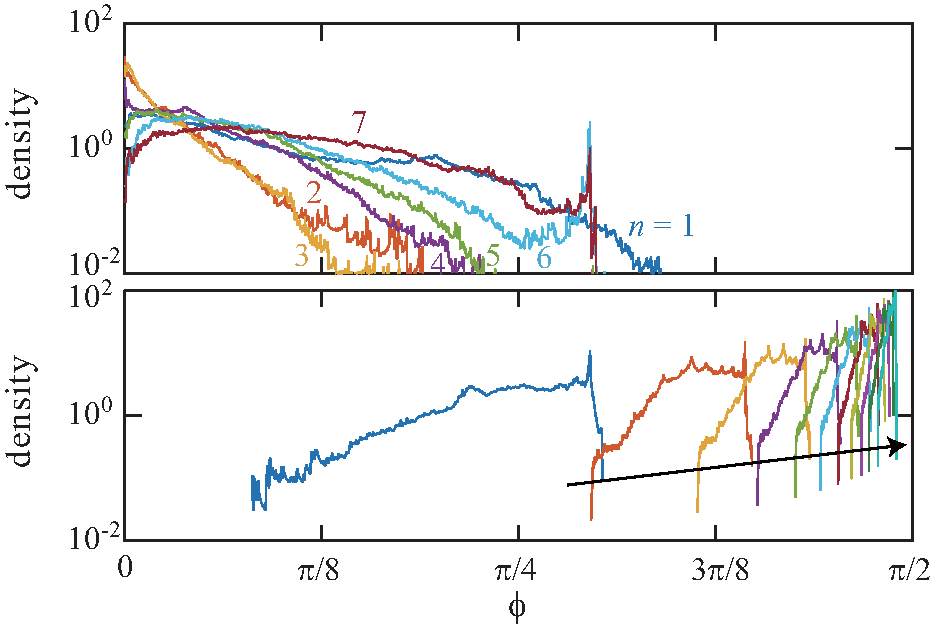
\includegraphics[width=0.9\textwidth]{ks22vecAngles}
  \caption[Principle angle density between subspaces formed by \Fv s]{
    %(Color online)
    A histogram of the principal angles $\phi$ between $S_n$
    (the subspace spanned by the $n$ leading \Fv s) and $\bar{S}_n$
    (the subspace spanned by the remaining $d-n$ \Fv s),
    accumulated over the 400 orbits used in our analysis. (top  panel) For
    $n=1,2,\cdots,7$ ($S_n$ within the \entangled\ manifold) the angles can be
    arbitrarily small. (bottom panel)
    For $n=8,10,12,\cdots,28$ (in the order of the arrow),
    for which all \entangled\ modes are contained in $S_n$,
    the angles are bounded away from unity.
  }
  \label{fig:ks22vecAngles}
\end{figure}

For an infinite-time chaotic trajectory, hyperbolicity can be assessed by
measuring the distribution of minimal principal
angles\rf{BjoGol73,Knyazev02} between any pair of subspaces spanned by
Lyapunov vectors\rf{ginelli-2007-99,YaTaGiChRa08,TaGiCh11}.
For any two subspaces $U$ and $V$, the $k$th principal angle
$\theta_k$ is defined as $\cos(\theta_k) = \max (u^\top v)$. Here,
$u$ and $v$ are two normalized vectors in $U$ and $V$ and
are subject to restriction $u^\top u_i = 0\,, v^\top v_i = 0$ for
$i = 1,\ldots,k-1$. Here, $u_i$ and $v_i$ achieve the $i$th principal
angle. Therefore, we can also write $\cos(\theta_k) = (u_k^\top v_k)$.
Principle angles provide information about the relative position of
these two subspaces in their embedding space. For our purpose, we are
only interested in the first principal angle which is the smallest
angle that can be formed by two arbitrary vectors from these two subspaces.
Let $U = Q_uR_u$ and $V = Q_vR_v$ be the QR decomposition of $U$ and $V$
respectively, then the first principal angle is given as
$\theta_1 = \arccos(\sigma_1)$, with $\sigma_1$ the smallest singular
value of $Q_u^\top Q_v$. In the following, whenever we say principal angle
$\theta$ or $\phi$, we shall be referring to the first principal angle.


Numerical work indicates that as the {\entangled} and {\transient} modes are
hyperbolically decoupled, the distribution of the angles between these
subspaces is bounded away from zero, and that observation yields a sharp
{\entangled}-{\transient} threshold.
This strategy cannot be used for individual orbits, as each one is of a
finite period, and the minimal principal angle reached by a pair of
Floquet subspaces remains strictly positive.
Instead, we measure the angle distribution for a \textit{collection} of
orbits, and find that the {\entangled}-{\transient} threshold is as sharp
as for a long chaotic trajectory: \reffig{fig:ks22vecAngles} shows the principal angle
distribution between two subspaces $S_n$ and $\bar{S}_n$, with $S_n$
spanned by the leading $n$ \Fv s and $\bar{S}_n$ by the rest.
As in the Lyapunov analysis of long chaotic trajectories\rf{YaTaGiChRa08}, the
distributions for small $n$ indicate strictly positive density as
$\phi\to0$. In contrast, the
distribution is strictly bounded away from zero angles for $n\geq 8$,
the number determined above by the local Floquet exponents analysis.
This leads to our second surmise:
(2) the distribution of principal angles for collections of \po s enables
us to identify a finite set of {\em {\entangled} Floquet modes}, the
analogue of the chaotic trajectories'  {\entangled} \cLv\ modes.

\subsection{Shadowing controlled by \Fv s}

\begin{figure}[!ht]
  \centering
  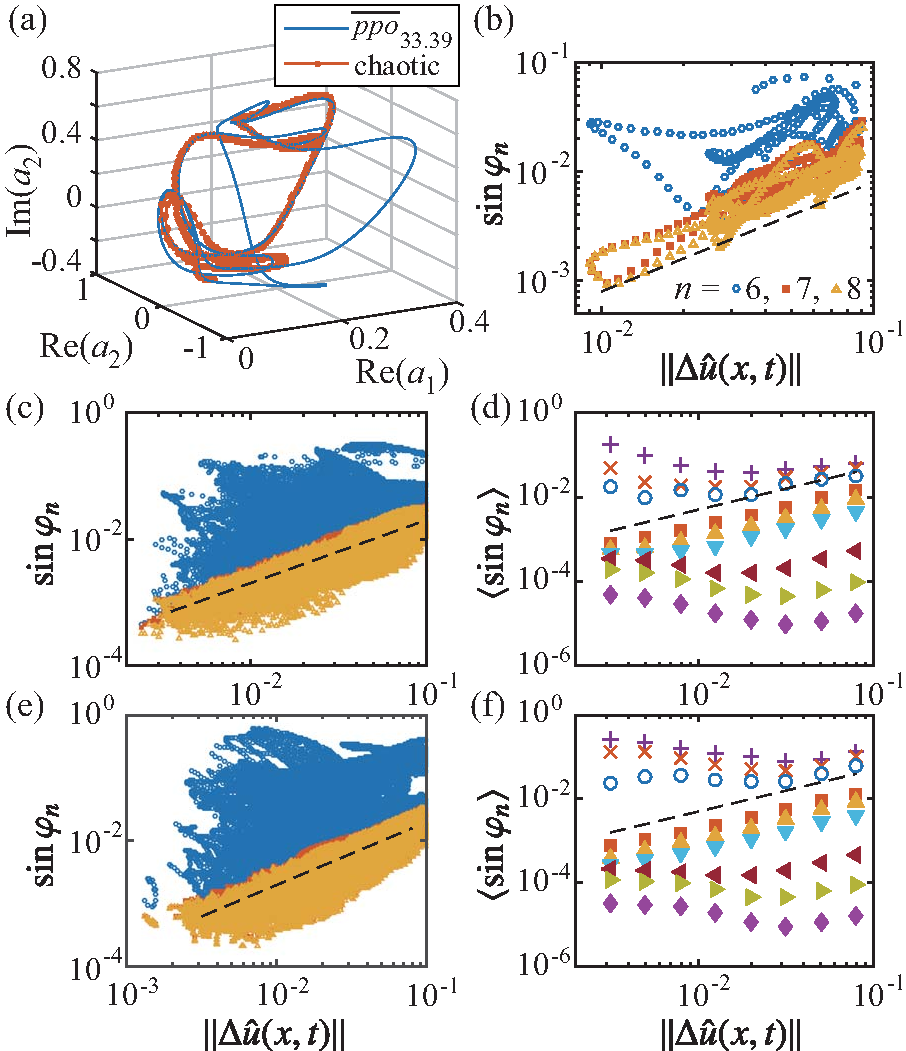
\includegraphics[width=0.9\textwidth]{ks22vecShadow}
  \caption[Separation vector spanned by \Fv s.]{
    (a) Shadowing event between a chaotic trajectory and $\overline{ppo}_{33.39}$,
    drawn over $2\,\period{p}$.
    (b) Parametric plot of $\sin\varphi_n(t)$ vs $||\Delta\hat{u}(x,t)||$
    during the single shadowing event shown in (a), for $n=6,7,8$.
    (c) Same as (b), but a total of 230 shadowing events of $\overline{ppo}_{33.39}$ are used.
    (d) Average of $\sin\varphi_n$ in (c),
    taken within each bin of the abscissa,
    for $n=4,5,6,7,9,11,17,21,25$ from top to bottom.
    (e)(f) Same as (c)(d), respectively,
    but for 217 shadowing events with $\overline{rpo}_{34.64}$.
    The dashed lines show $\sin\varphi_n\propto||\Delta\hat{u}||$ in all panels.
  }
  \label{fig:ks22vecShadow}
\end{figure}

It is known, at least for low\dmn\ chaotic systems, that a
dense set of \po s constitutes the skeleton of a strange
attractor\rf{DasBuch}. Chaotic trajectories meander around these orbits,
approaching them along their stable manifolds, and leaving them along their unstable
manifolds. If
trajectories are indeed confined to a
finite\dmn\ physical manifold, such shadowing events should take
place within the subspace of {\entangled} Floquet modes of the
shadowed orbit.
To analyze such shadowing, we
need to measure the distances between the chaotic trajectories and the
invariant orbits. But due to \SOn{2} symmetry, such shadowing
actually happens between two tori,
so we work in the 1st mode slice \refeq{eq:ksslice} defined in
\refsect{sect:kssym} to investigate shadowing incidences.

The dimension of the \slice\ subspace is one less than that of
the full \statesp:
\slice\ eliminates the marginal translational direction, while the
remaining Floquet multipliers $\Lambda_j$ are unchanged.
Therefore, for the system studied here, there are only seven {\entangled}
modes, with one marginal mode (time invariance) in the in-slice
description, instead of eight and two, respectively, in the full
\statesp\ description. Although we calculate \Fv s in the full \statesp,
relation \refeq{eq:Jrposlice} tells us how to get in-slice \Fv s
from \Fv s in the full \statesp.

A shadowing of
an orbit $u_{p}(x,t')$ by a nearby chaotic trajectory $u(x,t)$ is
then characterized by the in-slice separation vector
\begin{equation}
  \label{eq:dif}
  \Delta \hat{u}(x,t) \equiv \hat{u}(x, t) -\hat{u}_{p}(x, t_{p}),
\end{equation}
where $t_{p}$ is chosen to minimize the in-slice distance
$||\Delta\hat{u}||$.
Now we test whether the $\Delta{}\hat{u}(x,t)$ is
confined to the tangent space spanned by the {\entangled} in-slice Floquet
vectors. To evaluate this confinement, one needs to take into account the
nonlinearity of the stable and unstable manifolds for finite
amplitude of $\Delta\hat{u}(x,t)$.
We decompose the separation vector as
\begin{equation}
  \Delta\hat{u}(x,t)=\hat{v}_n(x,t)+\hat{w}_n(x,t),  \label{eq:DiffVec}
\end{equation}
where $\hat{v}_n(x,t)$ is a vector in the subspace $\hat{S}_n$ spanned by
the leading $n$ in-slice \Fv s and $\hat{w}_n(x,t)$ is in
the orthogonal complement
of $\hat{S}_n$. If $n$ is large enough so that $\hat{S}_n$
contains the local approximation of the inertial manifold, we expect
$||\hat{w}_n||\sim||\hat{v}_n||^2\sim||\Delta\hat{u}||^2$ because of the
smoothness of the inertial manifold;
otherwise $||\hat{w}_n||$ does not vanish as $||\Delta\hat{u}||\to{}0$.
In terms of the angle $\varphi_n$ between $\hat{S}_n$ and
$\Delta\hat{u}$,
$\sin\varphi_n\sim||\hat{w}_n||/||\hat{v}_n||\sim||\Delta\hat{u}||$ for
$n$ above the threshold, while $\sin\varphi_n$ remains non-vanishing
otherwise.


Following this strategy, we collected segments of a long chaotic
trajectory during which it stayed sufficiently close to a specific orbit
for at least one period of the orbit. \refFig{fig:ks22vecShadow}\,(a)
illustrates such a shadowing event for
\PPO{33.39}. A parametric plot of $\sin\varphi_n(t)$ vs.
$||\Delta\hat{u}(x,t)||$ during this event is shown in
\reffig{fig:ks22vecShadow}\,(b) for $n=6,7,8$ (blue circles, red squares,
orange triangles, respectively). We can already speculate from such a
single shadowing event that $\sin\varphi_n$ does not necessarily decrease
with $||\Delta\hat{u}||$ for $n<7$, while it decreases linearly with
$||\Delta\hat{u}||$ for $n\geq7$. This threshold is clearly identified by
accumulating data for all the recorded shadowing events with
\PPO{33.39}, \reffig{fig:ks22vecShadow}\,(c):
$\sin\varphi_n$ is confined below a line that depends linearly on
$||\Delta\hat{u}||$ if and only if $n\geq7$. Similarly, there is
a clear
separation in the average of $\sin\varphi_n$ taken within each bin of the
abscissa [\reffig{fig:ks22vecShadow}\,(d)]. This indicates that for $n<7$
(empty symbols), typical shadowing events manifest significant deviation
of $\Delta\hat{u}$ from the subspace $\hat{S}_n$, whereas for $n\geq7$
(solid symbols) $\Delta\hat{u}$ is always confined to $\hat{S}_n$. We
therefore conclude that shadowing events are confined to the subspace
spanned by the leading 7 in-slice \Fv s, or equivalently, by
all the 8 {\entangled} \Fv s in the full \statesp. The
same conclusion was drawn for \RPO{34.64}
[\reffig{fig:ks22vecShadow}\,(e) and (f)] and five other orbits
(not shown). We also verified that, when a chaotic trajectory approaches
an orbit, the subspace spanned by all {\entangled} Floquet modes of the
orbit coincides with that spanned by all {\entangled} Lyapunov modes of
the chaotic trajectory. This implies our third surmise: (3) the {\entangled}
Floquet manifold coincides locally with the {\entangled} Lyapunov
manifold, with either capturing the local structure of the inertial
manifold.

\subsection{Summary}
In summary, we used the \KS\ system to demonstrate by six
independent calculations that the tangent space of a dissipative flow
splits into \entangled\ vs. \transient\ subspaces, and to determine the
dimension of its inertial manifold. The \emph{Lyapunov modes} approach of
\refrefs{ginelli-2007-99,YaTaGiChRa08,YaRa11,TaGiCh11} identifies
(1) the ``\entangled'' Lyapunov exponents, by the dynamics of
finite-time Lyapunov exponents, \eqref{eq:ftle}; and
(2) the ``\entangled'' tangent manifold, or ``physical manifold,''
by measuring the distributions of angles between {\cLvs}.
The \emph{Floquet modes} approach\rf{DingCvit14} developed here shows that
(3) Floquet exponents of each \emph{individual} orbit separate into
\entangled\ vs. \transient, \refFig{fig:ks22FloqExp};
(4) for ensembles of orbits, the principal angles between hyperplanes
spanned by \Fv s separate the tangent space into \entangled\
vs. \transient, \reffig{fig:ks22vecAngles};
(5) for a chaotic trajectory shadowing a given orbit the separation
vector lies within the orbit's Floquet \entangled\ manifold,
\reffig{fig:ks22vecShadow}; and
(6) for a chaotic trajectory shadowing a given orbit the separation
vector lies within the
\cLvs' \entangled\ manifold.

All six approaches yield the same inertial manifold dimension, reported
in earlier work\rf{YaRa11}.
\footnote{
  see footnote \ref{fn:KazzNt1} on page \pageref{fn:KazzNt1}.
}
The Floquet modes / unstable \po s approach is constructive, in
the sense that periodic points should enable us, in principle (but not
attempted in this thesis), to tile the global inertial manifold by
local tangent spaces of an ensemble of such points.
Moreover, and somewhat surprisingly, our results on individual orbits'
Floquet exponents, \reffig{fig:ks22FloqExp}\,(b) and (c), and on
shadowing of chaotic trajectories, \reffig{fig:ks22vecShadow}, suggest
that \textit{each individual orbit} embedded in the attracting set
contains sufficient information to determine the
{\entangled}-{\transient} threshold.
However, the computation and organization of unstable \po s is
still a major undertaking, and can currently be carried out only for
rather small computational domains\rf{SCD07,WiShCv15}.
The good news is that the {\entangled} Lyapunov modes
approach\rf{YaTaGiChRa08} suffices to determine the inertial manifold
dimension, as Lyapunov modes calculations only require averaging over
long chaotic trajectories, are much easier to implement, and can be
scaled up to much larger domain sizes than $L=22$ considered here.

We hope the computational tools
introduced here, namely, local Floquet exponents, principal angles obtained
by \Fv s, and expansion errors of difference vectors in shadowing incidences,
will eventually
contribute to solving outstanding issues of dynamical systems theory,
such as the existence of an inertial manifold in the transitional
turbulence regime of the \NSe.
